\chapter{Stand van zaken}
\label{ch:stand-van-zaken}

% Tip: Begin elk hoofdstuk met een paragraaf inleiding die beschrijft hoe
% dit hoofdstuk past binnen het geheel van de bachelorproef. Geef in het
% bijzonder aan wat de link is met het vorige en volgende hoofdstuk.

% Pas na deze inleidende paragraaf komt de eerste sectiehoofding.

Dit hoofdstuk is een literatuurstudie over de huidige stand van zaken rond Kotlin. Wat is Kotlin, Kotlin en Android, Kotlin en iOS, Kotlin en cross-platform development, Kotlin Native, LLVM en het gebruik van Kotlin. Na het lezen van dit hoofdstuk bent u volledig op de hoogte van de laatste updates van Kotlin.

\section{Wat is Kotlin}
\label{sec:kotlin}
Kotlin is een open-source programmeertaal die object-georiënteerde en functioneel programmeer features combineert. Kotlin is ook een static type programmeertaal. Dit betekent dat variabelen niet moeten gedefinieerd worden alvorens men deze gebruikt. Anders gezegd, het type van de variabele is gekend wanneer de code wordt gecompileerd.

Deze programmeertaal is ontworpen door JetBrains. JetBrains is een software ontwikkeling bedrijf dat gesticht is in het jaar 2000. Hun hoofdkantoor is gevestigd in Praag, Tjsechië. Hun core-business is het ontwikkelen van tools die gebruikt kunnen worden door verschillende types van software ontwikkelaars. Zo hebben zij IDE's \footnote{Integrated Development Environment} ontwikkeld voor Java, Ruby, Python, PHP, SQL, Objective-C, C++, C\# en JavaScript.

\section{Kotlin en Android}
\label{sec:kotlinandroid}
In 2017 heeft Google bekend gemaakt dat het Kotlin volledig zou ondersteunen voor Android. Een Kotlin project maken in Android Studio is dan ook heel gemakkelijk. Je begint best met het installeren van de Kotlin plugin. Daarna maak je een nieuw Android Studio project aan. Origineel zal dit nog geschreven zijn in Java. 
Automigration


\section{Kotlin web en back-end}
\label{sec:kotlincrossplatform}
https://kotlinlang.org/docs/tutorials/httpservlets.html
https://kotlinlang.org/docs/reference/server-overview.html
https://medium.com/bcgdv-engineering/building-a-full-stack-web-app-in-kotlin-af8e8fe1f5dc

\section{Kotlin Native}
\label{sec:kotlinnative}
https://kotlinlang.org/docs/reference/native-overview.html

\section{LLVM}
\label{sec:llvm}
https://blog.jetbrains.com/kotlin/2017/04/kotlinnative-tech-preview-kotlin-without-a-vm/

\section{Het gebruik van Kotlin}
\label{sec:kotlingebruik}
Het gebruik van Kotlin is gedurende de jaren zeer sterk gestegen. Op de blog van JetBrains zijn grafieken te vinden waarmee men aantoont dat de populariteit van Kotlin enkel maar stijgt.

\begin{figure} [ht]
	\centering
	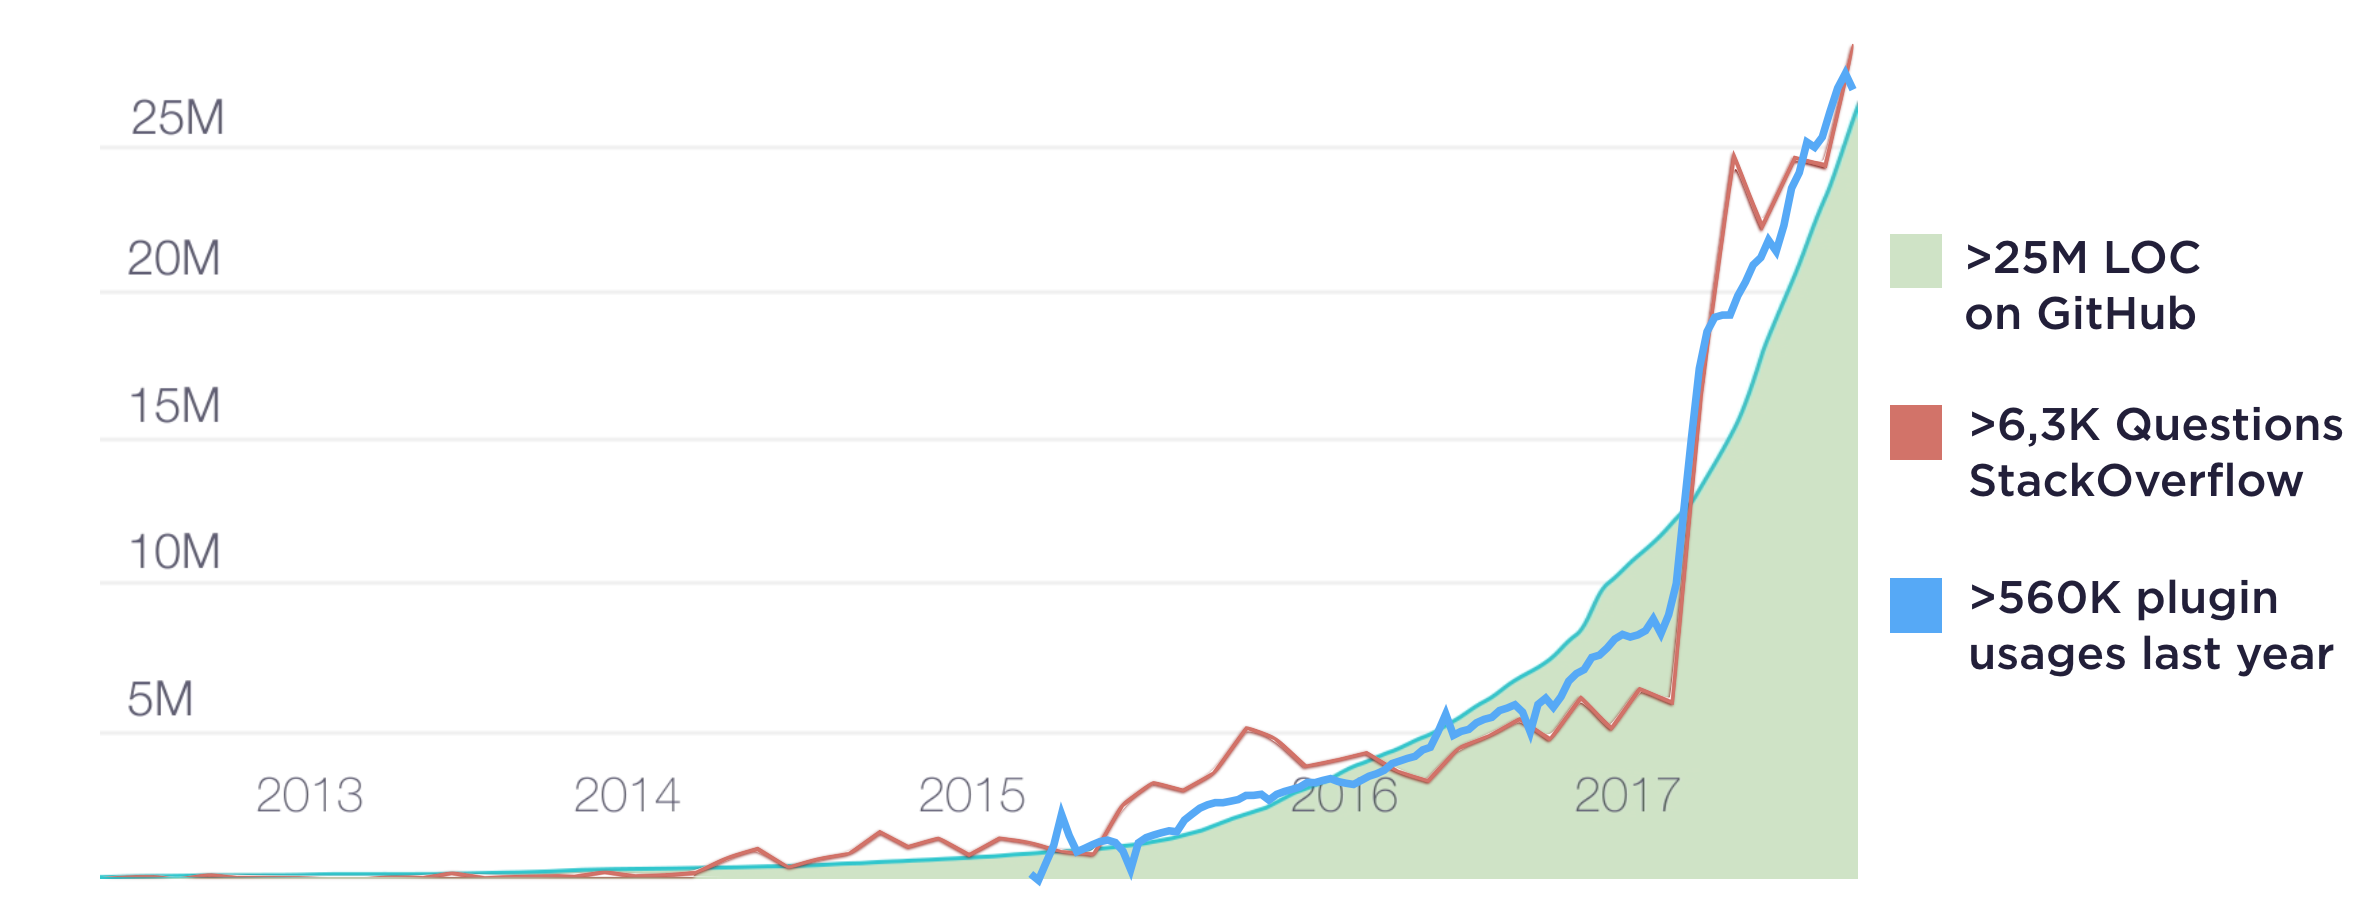
\includegraphics[width=0.95\textwidth]{img/KotlinAdoption.png}
	\caption{Hoeveelheid Github code in Kotlin \cite{JetBrains12}}
	\label{fig:kotlingithub}
\end{figure}

Deze tweede figuur toont de verschillende user groups over de volledige wereld. Het toont aan dat Kotlin toch zeer veel gebruikt worden in onze streken.
\begin{figure} [ht]
	\centering
	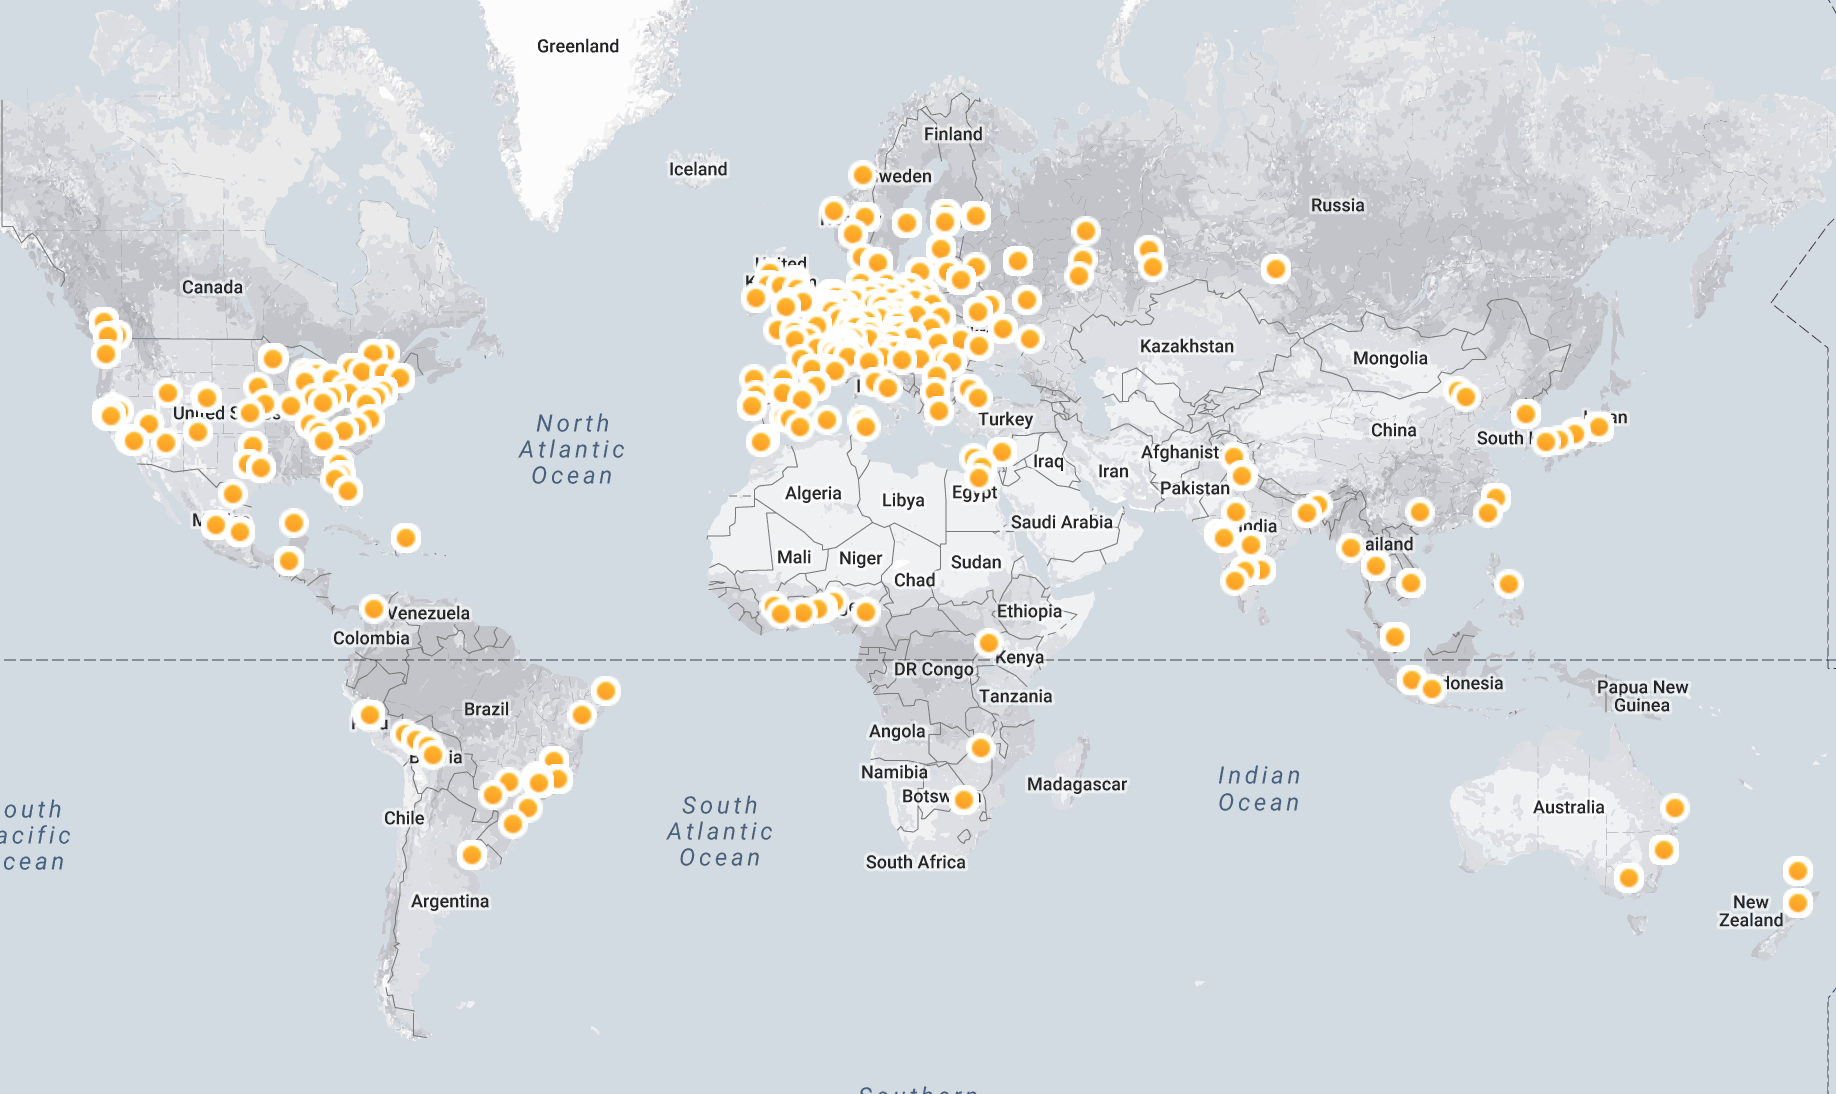
\includegraphics[width=0.95\textwidth]{img/KUGmap.png}
	\caption{User groups in de wereld \cite{JetBrains12}}
	\label{fig:usergroups}
\end{figure}


%Dit hoofdstuk bevat je literatuurstudie. De inhoud gaat verder op de inleiding, maar zal het onderwerp van de bachelorproef *diepgaand* uitspitten. De bedoeling is dat de lezer na lezing van dit hoofdstuk helemaal op de hoogte is van de huidige stand van zaken (state-of-the-art) in het onderzoeksdomein. Iemand die niet vertrouwd is met het onderwerp, weet er nu voldoende om de rest van het verhaal te kunnen volgen, zonder dat die er nog andere informatie moet over opzoeken \autocite{Pollefliet2011}.

%Je verwijst bij elke bewering die je doet, vakterm die je introduceert, enz. naar je bronnen. In \LaTeX{} kan dat met het commando \texttt{$\backslash${textcite\{\}}} of \texttt{$\backslash${autocite\{\}}}. Als argument van het commando geef je de ``sleutel'' van een ``record'' in een bibliografische databank in het Bib\TeX{}-formaat (een tekstbestand). Als je expliciet naar de auteur verwijst in de zin, gebruik je \texttt{$\backslash${}textcite\{\}}.
%Soms wil je de auteur niet expliciet vernoemen, dan gebruik je \texttt{$\backslash${}autocite\{\}}. In de volgende paragraaf een voorbeeld van elk.

%\textcite{Knuth1998} schreef een van de standaardwerken over sorteer- en zoekalgoritmen. Experten zijn het erover eens dat cloud computing een interessante opportuniteit vormen, zowel voor gebruikers als voor dienstverleners op vlak van informatietechnologie~\autocite{Creeger2009}.

%\lipsum[7-20]
